\chapter{RESULTADOS, DISCUSSÃO E LIMITAÇÕES}
\label{chapter-6}
\section{Funcionalidades observadas}
\label{section-6-1}
O artefato disponibiliza três perfis explícitos, calendário consultável, catálogo inicial de atos, memória, exportação e impressão. Conta, histórico privado e lembrete opcional foram integrados. A aplicação é web responsiva; não foi desenvolvido um aplicativo nativo nem um sistema de análise automática de documentos ou consulta a processos judiciais.

\begin{figure}[H]\centering
\caption{Resultado e avisos na interface publicada}
\label{figure-9}
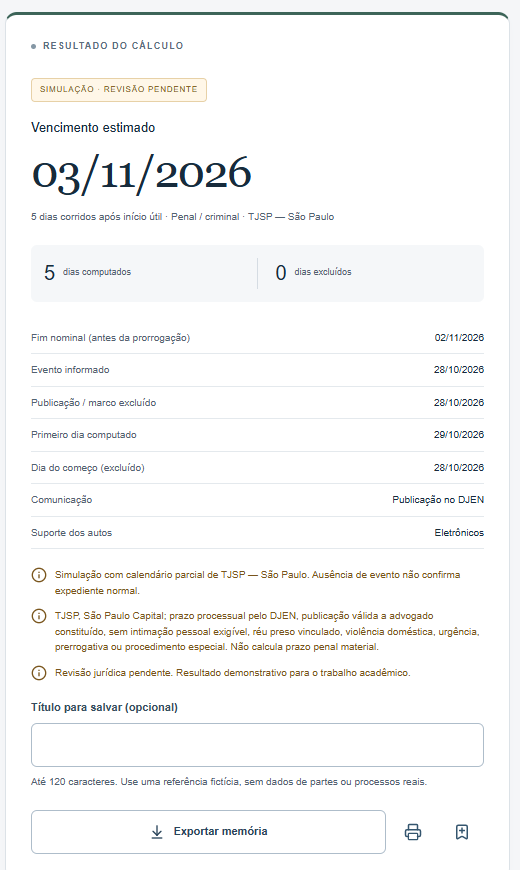
\includegraphics[width=\linewidth,height=.58\textheight,keepaspectratio]{figuras/tela-calculadora.png}
\par\smallskip{\fontsize{10}{12}\selectfont Fonte: captura da aplicação publicada em 23/10/2026, recorte do resultado; acervo do projeto.}
\end{figure}
A figura registra o aplicativo publicado em 23/10/2026. A versão funcional de 24/10 acrescentou a orientação dedicada após cadastro. A captura controlada a seguir mostra essa página sem dados reais de conta; sua existência não comprova a entrega de e-mail em uma execução particular.

\begin{figure}[H]\centering
\caption{Orientação após cadastro em teste controlado}
\label{figure-10}
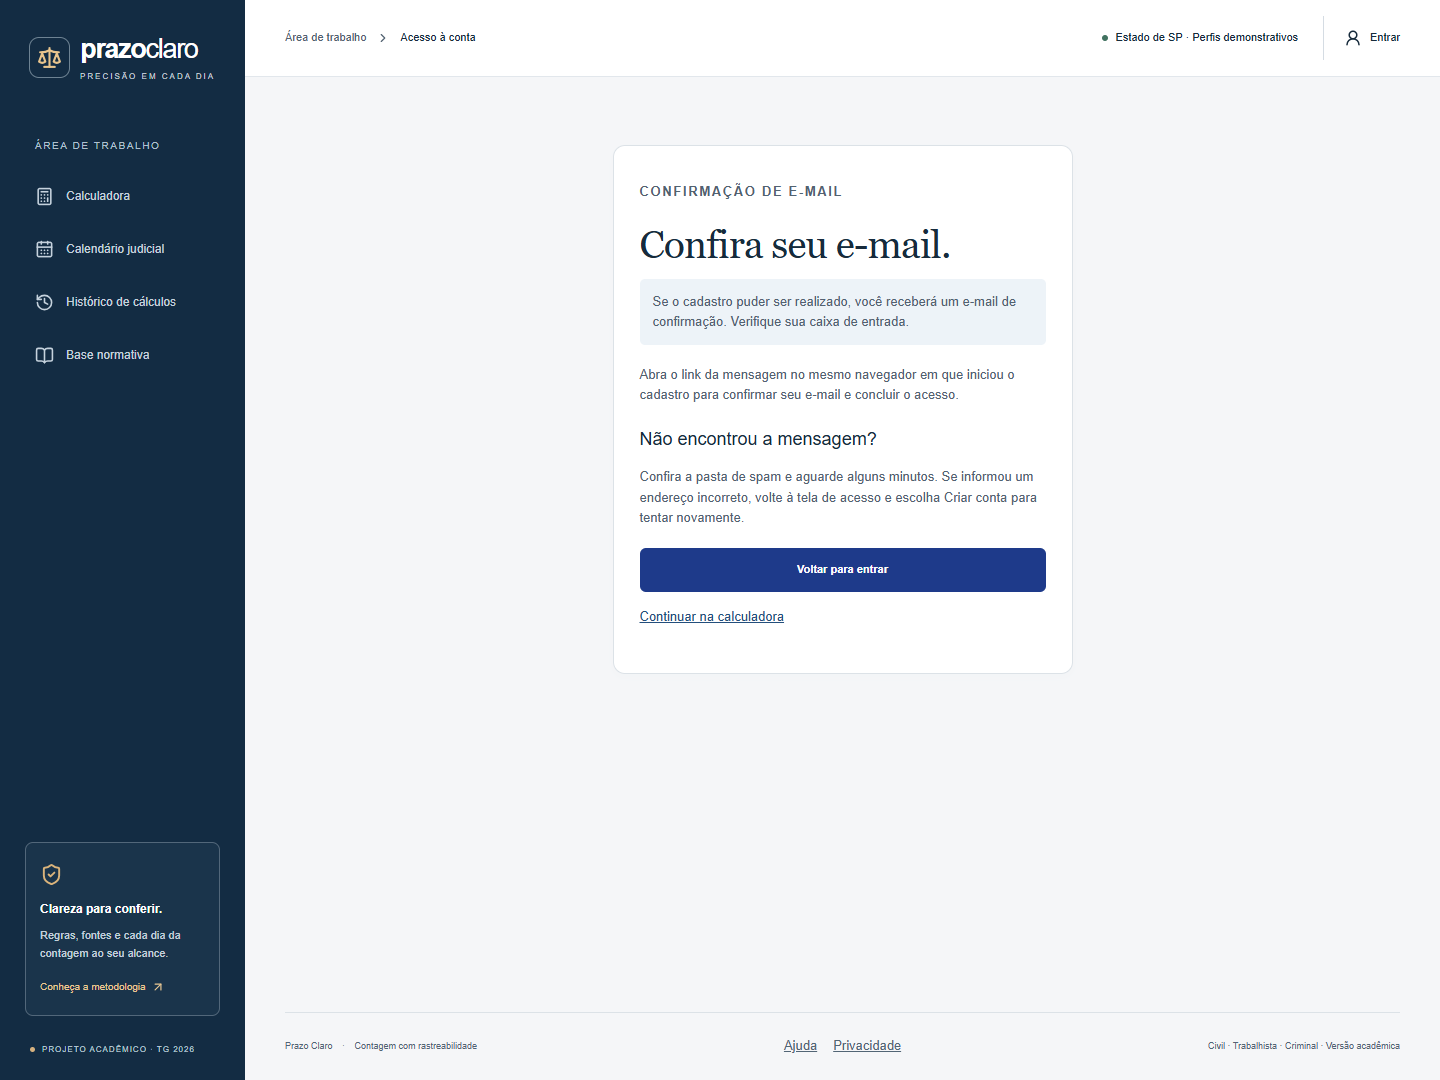
\includegraphics[width=\linewidth,height=.39\textheight,keepaspectratio]{figuras/tela-confirmacao.png}
\par\smallskip{\fontsize{10}{12}\selectfont Fonte: captura de teste controlado da aplicação, 24/10/2026; sem dados reais de conta.}
\end{figure}
\section{Casos de referência e rastreabilidade}
\label{section-6-2}
Os casos a seguir permitem comparar efeitos de perfil e localidade sob os dados demonstrativos. As datas são resultados técnicos das premissas registradas, sujeitos às lacunas do calendário e à revisão jurídica pendente. A mesma entrada numérica não autoriza transferir o resultado entre regimes.

\begin{quadro}[H]\centering
\caption{Casos demonstrativos de referência}
\label{quadro-3}
\begin{singlespace}\fontsize{10}{12}\selectfont
\begin{tabularx}{\linewidth}{|>{\raggedright\arraybackslash}X|>{\raggedright\arraybackslash}X|>{\raggedright\arraybackslash}X|}
\hline
\textbf{Perfil e local} & \textbf{Publicação e duração} & \textbf{Resultado esperado} \\
\hline
Civil TJSP Capital & 06/10/2026; 5 dias úteis & 14/10/2026 \\
\hline
Civil TJSP Santos & 04/09/2026; 1 dia útil & 09/09/2026 \\
\hline
Civil TJSP Capital & 04/09/2026; 1 dia útil & 08/09/2026 \\
\hline
Criminal TJSP Capital, ordinário & 06/10/2026; 5 dias processuais & 13/10/2026 \\
\hline
Trabalhista TRT-2 Capital, ordinário & 17/12/2026; 10 dias úteis & 03/02/2027 \\
\hline
TJSP fora da cobertura temporal & Travessia sem calendário suficiente & Incompleto, vencimento nulo \\
\hline
\end{tabularx}\end{singlespace}
\par\smallskip{\fontsize{10}{12}\selectfont Fonte: elaboração com base nos registros do projeto (2026).}
\end{quadro}
No primeiro caso, a trilha permite conferir 7, 8 e 9 de outubro, a exclusão do fim de semana e de 12 de outubro, e a continuação em 13 e 14. Nos casos de Santos e Capital, a diferença decorre da seleção municipal, não de uma alteração arbitrária da duração. Na travessia trabalhista, a memória identifica os dois componentes anuais e os períodos excluídos.

\section{Resultados automatizados e aceites humanos}
\label{section-6-3}
A CI 40061653068 foi aprovada na versão 9632fd2. O quadro separa verificações de código e banco de observações de uso. Não foi calculado percentual de cobertura de linhas nem desempenho sob carga; contagem de testes aprovados não equivale a essas métricas.

\begin{table}[H]\centering
\caption{Resultados registrados de verificação automatizada}
\label{tabela-1}
\begin{singlespace}\fontsize{10}{12}\selectfont
\begin{tabularx}{\linewidth}{>{\raggedright\arraybackslash}X>{\raggedright\arraybackslash}X>{\raggedright\arraybackslash}X}
\hline
\textbf{Categoria} & \textbf{Aprovados} & \textbf{Arquivos ou observação} \\
\hline
Unitários & 256 & 18 arquivos \\
SQL/pgTAP & 146 & 5 arquivos \\
Navegador E2E & 67 & 1 cenário omitido \\
\hline
\end{tabularx}\end{singlespace}
\par\smallskip{\fontsize{10}{12}\selectfont Fonte: elaboração com base nos registros do projeto (2026).}
\end{table}
Fonte: registros da CI 40061653068 e docs/testing/signup-confirmation-page.md, 24/10/2026. Tipos, lint, formatação e build também foram aprovados na execução identificada. O cenário omitido não foi contado como sucesso. Os totais agregam verificações de diferentes fronteiras e não devem ser somados como uma medida única de qualidade.

O responsável confirmou uso hospedado de Google com retorno conectado, cadastro com recebimento e confirmação de e-mail, entrada da nova conta, recuperação de senha, histórico após recarga e exportação. Esses relatos são aceites operacionais individuais, não uma pesquisa com amostra de usuários. O fluxo de convite possui integração local aprovada; o reensaio completo no ambiente hospedado permanece com aceite próprio.

\section{Situação do lembrete externo}
\label{section-6-4}
O ensaio de 24/10 às 09h foi inconclusivo. O responsável informou que não recebeu a mensagem e excluiu o cálculo, sem lembrar o horário. A fila vazia e a exclusão em cascata explicam a ausência atual do registro, mas não provam se o cancelamento ocorreu antes do horário. Portanto, não se afirma nem entrega bem-sucedida nem uma causa técnica de falha que os dados não permitem demonstrar.

Um novo agendamento foi conferido às 13h44 de 24/10 para 18h de São Paulo, com vencimento estimado em 27/10 e antecedência de três dias. Na conferência, o estado era pending, sem tentativa ou erro, com agendador ativo. Recebimento da mensagem e abertura da memória permaneciam pendentes no corte deste relatório. O registro deve ser mantido até concluir o ensaio; nenhum horário foi antecipado artificialmente para produzir uma evidência de sucesso.

\section{Análise dos objetivos e decisões}
\label{section-6-5}
O primeiro objetivo específico foi atendido tecnicamente pela especificação dos perfis, vocabulário e critérios de aceite, conservando fontes e lacunas. O segundo foi atendido pela separação do motor e pela integração de recursos privados, demonstrada em testes locais e uso hospedado. O terceiro foi atendido no âmbito da verificação técnica e da documentação; validação jurídica, avaliação com participantes e recebimento do novo lembrete continuam sem encerramento.

A principal decisão de projeto foi tornar a insuficiência de dados um resultado explícito. Isso reduz a aparência de cobertura universal, mas exige explicar ao usuário por que uma combinação não gera data. Outra decisão foi preservar motores e snapshots históricos, o que aumenta o custo de manutenção e evita modificar silenciosamente memórias antigas. O uso de serviços gerenciados simplificou a implantação, mas criou dependências de configuração, cotas e disponibilidade externas.

\section{Custos, riscos e validade}
\label{section-6-6}
Não houve levantamento financeiro com faturas nem apontamento completo de horas. Por isso, não se apresenta orçamento executado, retorno de investimento ou economia mensurada. As categorias relevantes são hospedagem, banco e autenticação, envio transacional, eventual domínio, manutenção técnica e revisão jurídica. Planos gratuitos usados na demonstração não constituem garantia permanente de custo zero ou de capacidade para uso institucional.

As ameaças à validade incluem a cobertura parcial dos calendários, a revisão jurídica ausente, a participação concentrada no responsável do projeto e os testes de interface com respostas simuladas. Dependências e regras podem mudar após o corte. A execução em CI amplia a repetibilidade técnica, mas não comprova todas as configurações do ambiente hospedado. Aceite do provedor não prova chegada à caixa de entrada, e ausência de dados após exclusão limita diagnóstico retrospectivo.

A auditoria de dependências contém mitigação específica documentada para braces; saída de sucesso não representa ausência universal de vulnerabilidades. Não foram executados estudo SUS, pesquisa de campo, teste amplo de carga, auditoria independente ou restauração institucional completa. Esses itens não aparecem como gráficos ou tabelas com valores inventados.

\section{Continuidade priorizada}
\label{section-6-7}
O fechamento imediato requer concluir o ensaio externo do lembrete, reensaiar convite hospedado e apresentação, revisar este relatório pela autora e orientação e conferir os anexos acadêmicos exigidos. Em seguida, devem ser priorizados revisão jurídica e levantamento completo das unidades e suspensões do recorte escolhido, antes de expandir tribunais ou afirmar uso profissional.

A evolução técnica inclui política de retenção e atendimento, backup e restauração ensaiados, controle distribuído de abuso, observabilidade e governança de segredos. Funcionalidades como equipes, cadastro completo de processos, administração normativa e novos meios de comunicação dependem de requisitos e testes próprios. Ampliar apenas um seletor visual não resolve essas lacunas.
